\section{Medição da chuva}

A medição do volume de chuva ocorre há milhares de anos. Os registros mais antigos de que se têm conhecimento foram feitos na Grécia por volta de 500 a.C. Para medir a quantidade de precipitação por unidade de superfície, durante certo intervalo de tempo, utiliza-se o pluviômetro ou pluviógrafo. A medição é expressa em milímetros de altura de chuva ($mm$) ou em litros por metro quadrado ($L/m^2$) \cite{site-chuva}.

No Sistema Internacional de Unidades, a unidade de pluviosidade é o milímetro. A pluviosidade de 1 milímetro equivale ao volume de 1 litro de água que precipitou em 1 metro quadrado. A relação entre litros por metro quadrado e milímetro é apresentada na Equação \ref{eq:relacao}.

\begin{equation}
\label{eq:relacao}
    \frac{1L}{m^2} = \frac{1 dm^3}{m^2} \Longleftrightarrow\frac{(1 dm)^3}{m^2} = \frac{10^{-3}m^3}{m^2} = 10^{-3} m = 1mm
\end{equation}

\subsection{Pluviômetro}
As medições das precipitações de chuvas são realizadas com a utilização de um pluviômetro, representado na Figura \ref{fig:pluviometro}, aparelho com medidas normalizadas em formato cilíndrico que, exposto às intempéries, reserva a água da chuva precipitada entre um intervalo de leituras. Uma proveta graduada permite a leitura do volume de água acumulado dentro do medidor. O volume de água, dividido pela área de captação do pluviômetro, resulta em uma altura análoga de chuva, definida em milímetros. As leituras devem ser realizadas diariamente, sempre no mesmo horário \cite{manual-daee}.

\begin{figure}[h]
    \caption{Pluviômetro da Estação Meteorológica do IAG-USP}
    \centering
    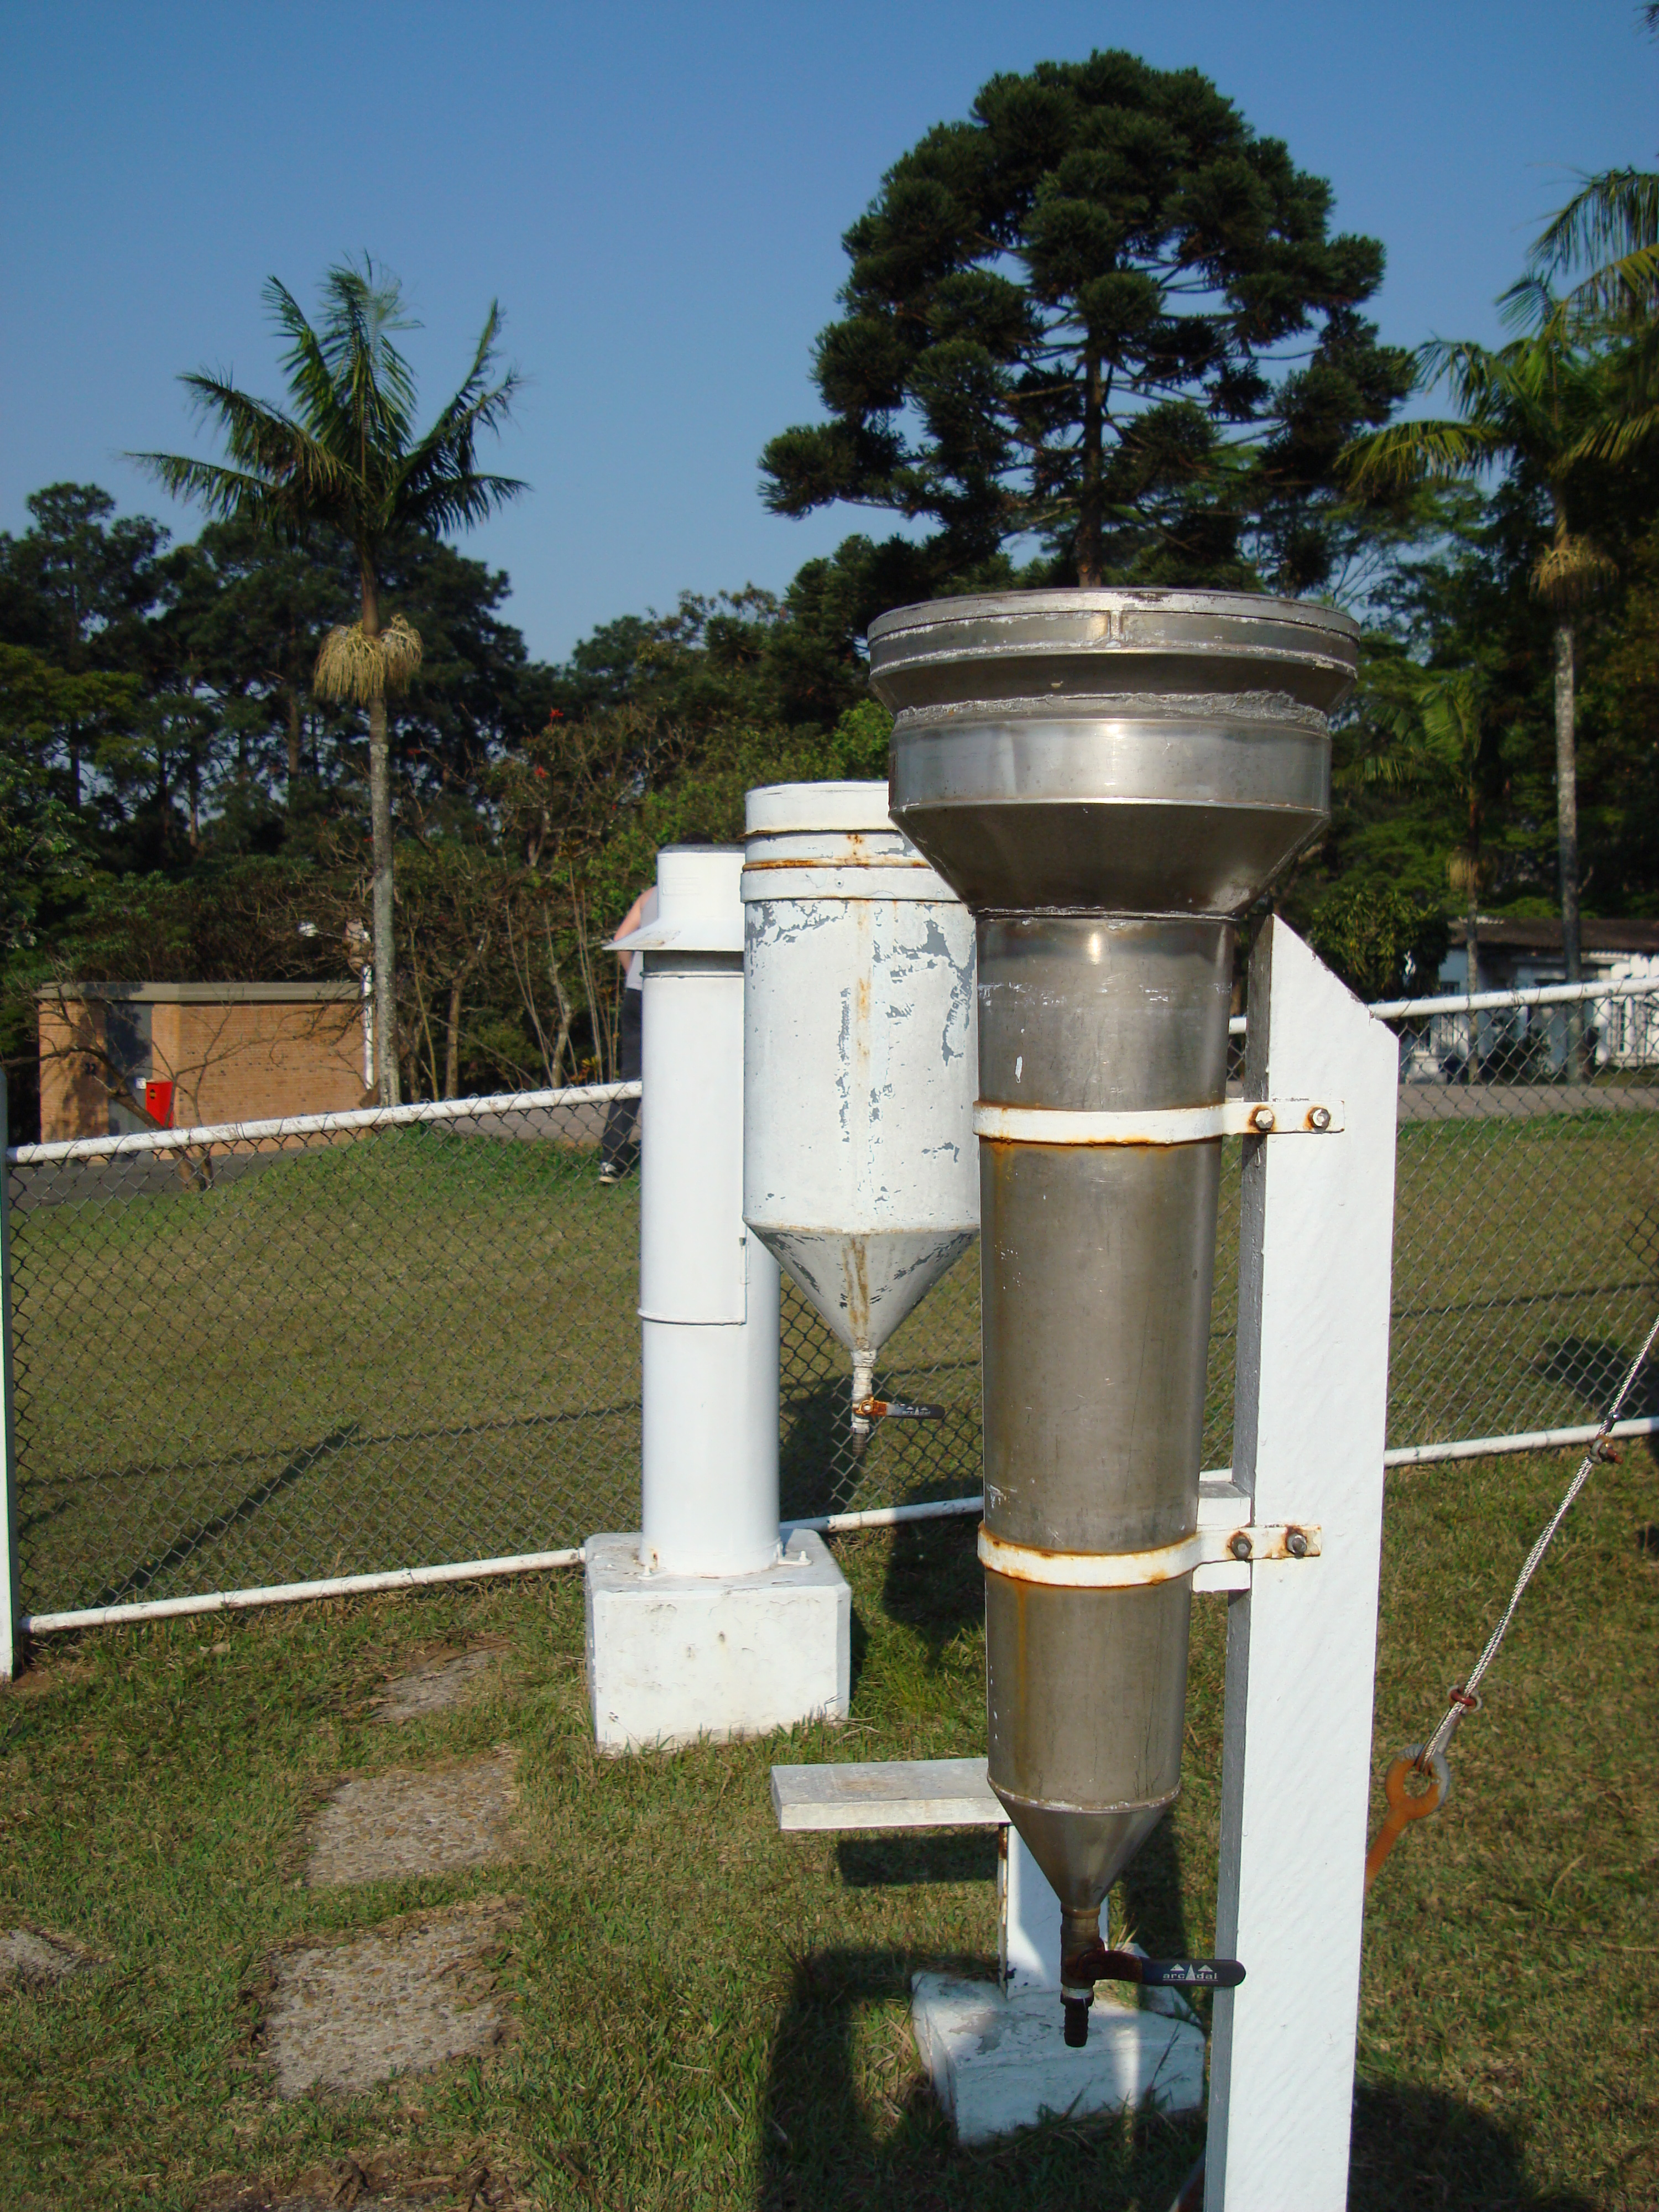
\includegraphics[width=0.35\textwidth, keepaspectratio]{Textuais/Figuras/pluviometro.jpg}
    \fonte{http://meteoropole.com.br/2011/12/o-que-e-um-pluviometro}
    \label{fig:pluviometro}
\end{figure}


\subsection{Pluviógrafo}

Outro tipo de medidor de chuvas é o Pluviógrafo representado na Figura \ref{fig:pluviografo}. Existe uma grande variedade de aparelhos, usando princípios diferentes para medir e gravar continuamente o registro das chuvas. Os pluviógrafos permitem medir as intensidades das chuvas durante intervalos de tempo menores àqueles obtidos com as observações manuais feitas nos pluviômetros \cite{tucci1993}.

\begin{figure}[h]
    \caption{Representação de um pluviógrafo}
    \centering
    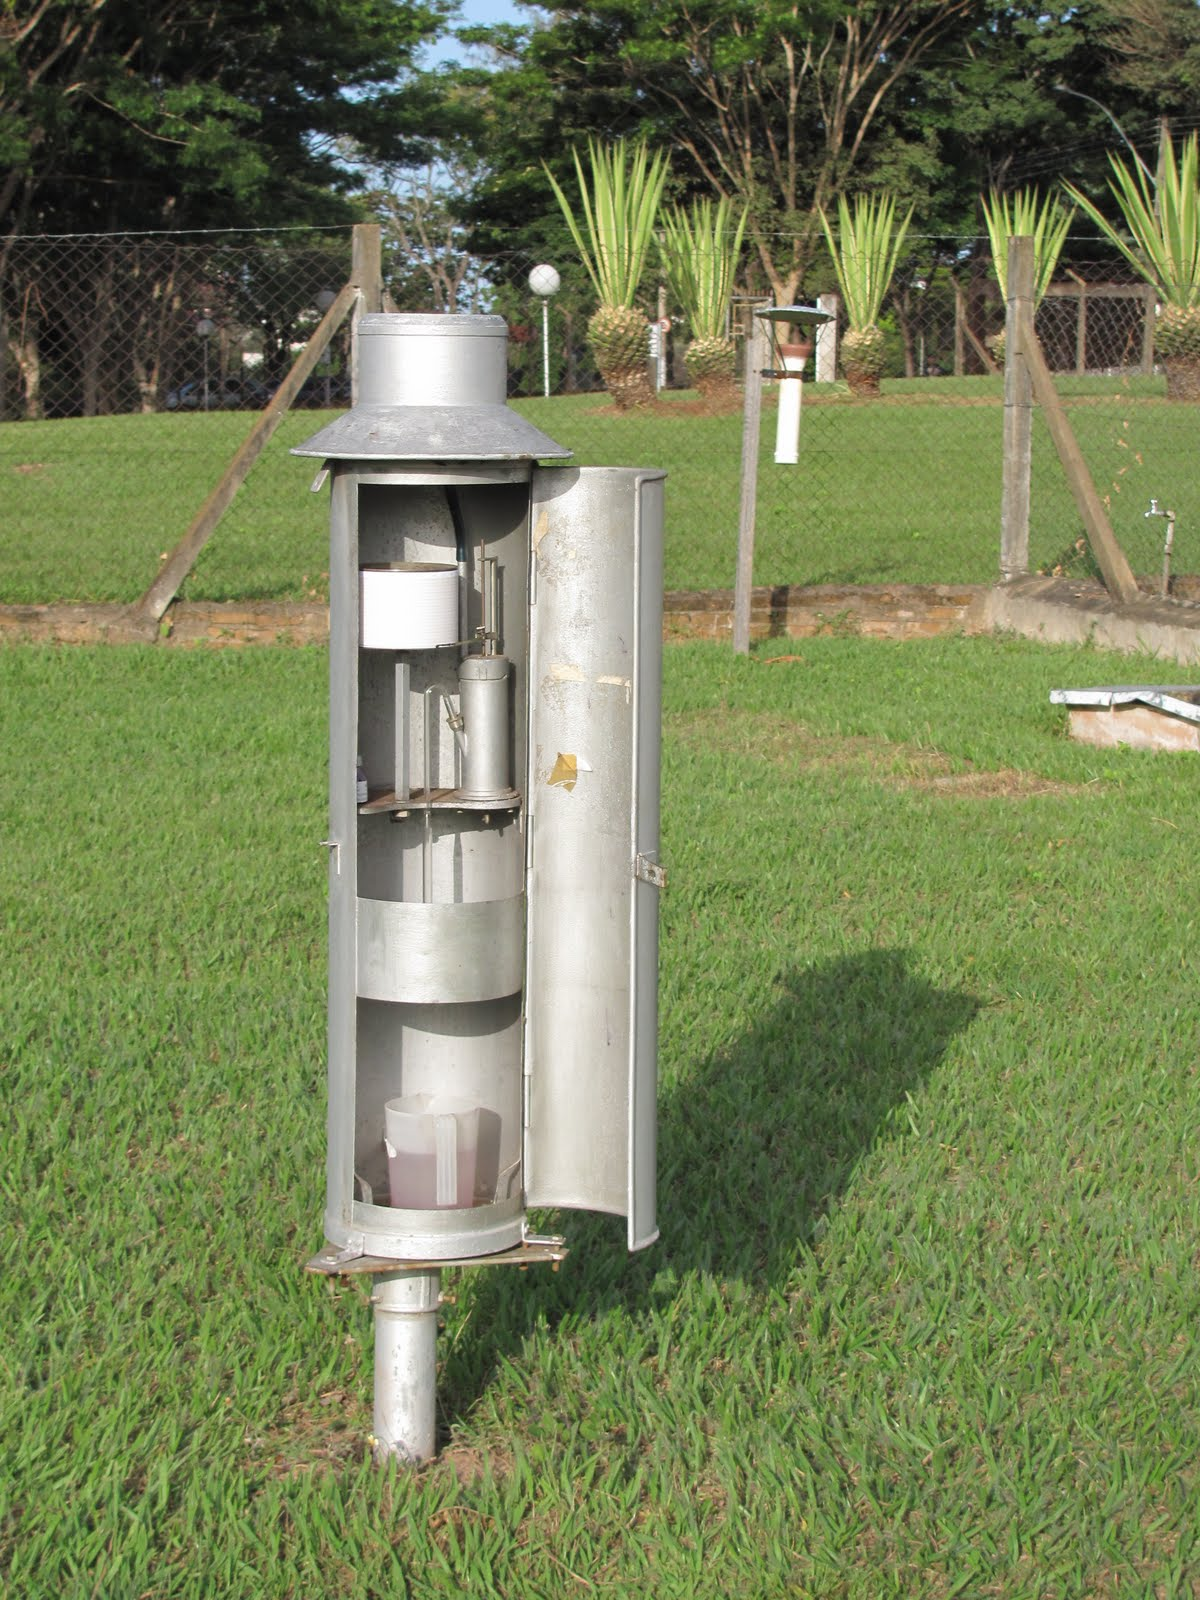
\includegraphics[width=0.35\textwidth, keepaspectratio]{Textuais/Figuras/pluviografo.jpg}
    \fonte{http://estacaometeorologicafctunesp.blogspot.com/2011/06/pluviografo.html}
    \label{fig:pluviografo}
\end{figure}

\section{Distribuição dos aparelhos de medição em Pernambuco}

\citeonline{analise-pernambuco} disponibiliza os relatos que compuseram a história e desenvolvimento da rede de hidrometria no estado de Pernambuco, como será apresentado brevemente a seguir.

A região Nordeste conta com 1225 postos pluviométricos em funcionamento, dos quais 149 estão no estado de Pernambuco. Alguns operam somente há poucos meses ou um pouco mais, outros funcionaram por alguns anos e foram desativados, e em uma última parcela, pôde-se constatar séries contínuas de muitos postos com mais de 40 anos de registros pluviométricos \cite{analise-pernambuco}.

Essas redes de medições de postos foram mantidas no estado de Pernambuco por diversas instituições e registrou séries históricas. As quantidades de postos operados por cada instituição foram: 75 pelo Departamento Nacional de Obras Contra a Seca (DNOCS); 24 pelo Serviço de Meteorologia Nacional (CPRM); 4 pela Divisão de Águas e 46 por entidades privadas. Na época também foram instalados 4 pluviógrafos dos 37 existentes no Nordeste, que equivalem a 3\% dos 149 instalados em Pernambuco \cite{analise-pernambuco}.

Em 1960 iniciou-se a fase que foi caracterizada pela criação da Superintendência de Desenvolvimento do Nordeste - SUDENE e a reestruturação da rede. A SUDENE publicou diversos trabalhos sobre dados pluviométricos, tal como ``Dados Pluviométricos mensais do Nordeste``, sendo o sexto volume dedicado ao estado de Pernambuco \cite{analise-pernambuco}.

Ainda de acordo com \citeonline{analise-pernambuco}, o estado de Pernambuco, no ano de 2003, contava com uma rede com um total de 375 estações operadas simultaneamente por entidades Federais e Estaduais, cuja densidade decrescia no sentido Litoral ao Sertão, segundo informações das próprias entidades. A Tabela \ref{tab:estacoes} apresenta as quantidades de estações funcionais no estado de Pernambuco em 2003.

\begin{table}[htbp]
\centering
\caption{Estações de medição operadas em 2003 no estado de Pernambuco}
\begin{tabular}{@{}cc@{}}
\toprule
Órgão Operador & Número de Pluviômetros \\ \midrule
ANA            & 40                     \\
INMET          & 11                     \\
SECTMA         & 222                    \\
COMPESA        & 13                     \\
IPA / EBAPE    & 82                     \\
INFRAERO       & 02                     \\
EMBRAPA        & 04                     \\
CHESF          & 01                     \\ \midrule
Total          & 375                    \\ \bottomrule
\end{tabular}
\fonte{\citeonline{analise-pernambuco}}
\label{tab:estacoes}
\end{table}